% This file compiles on a standard distribution of LaTeX (say, TeXLive)
% The PDF file it generates is in ./LaTeX/ConsumptionResponse.pdf
% LaTeX path to the root directory of the current project
\providecommand{\econtexRoot}{}
\renewcommand{\econtexRoot}{.}
% The \commands below are required to allow sharing of the same base code via Github between TeXLive on a local machine and ShareLaTeX.  This is an ugly solution to the requirement that custom LaTeX packages be accessible, and that ShareLaTeX seems to ignore symbolic links (even if they are relative links to valid locations)
\providecommand{\econtex}{\econtexRoot/LaTeX/texmf-local/tex/latex/econtex}
\providecommand{\econtexSetup}{\econtexRoot/LaTeX/texmf-local/tex/latex/econtexSetup}
\providecommand{\econtexShortcuts}{\econtexRoot/LaTeX/texmf-local/tex/latex/econtexShortcuts}
\providecommand{\econtexBibMake}{\econtexRoot/LaTeX/texmf-local/tex/latex/econtexBibMake}
\providecommand{\econtexBibStyle}{\econtexRoot/LaTeX/texmf-local/bibtex/bst/econtex}
\providecommand{\notes}{\econtexRoot/LaTeX/texmf-local/tex/latex/handout}
\providecommand{\handoutSetup}{\econtexRoot/LaTeX/texmf-local/tex/latex/handoutSetup}
\providecommand{\handoutShortcuts}{\econtexRoot/LaTeX/texmf-local/tex/latex/handoutShortcuts}
\providecommand{\handoutBibMake}{\econtexRoot/LaTeX/texmf-local/tex/latex/handoutBibMake}
\providecommand{\handoutBibStyle}{\econtexRoot/LaTeX/texmf-local/bibtex/bst/handout}
\providecommand{\economics}{economics}
\documentclass[titlepage,a4paper]{\econtex}

\provideboolean{ifIJCB}\setboolean{ifIJCB}{false} % If true, make IJCB version, otherwise regular
\provideboolean{ifECB}\setboolean{ifECB}{false} % If true, make ECB version, otherwise regular
\providecommand{\versn}{}
\ifthenelse{\boolean{ifIJCB}}{\renewcommand{\versn}{IJCB}}{} % Includes in tiny header 

\providecommand{\texname}{ConsumptionResponse}% Keyname for the bibtex entry corresponding to this paper

\usepackage{\econtexRoot/LaTeX/ConsumptionResponse} % defines ifWeb among other things

\ifthenelse{\boolean{ifIJCB}}{ 
    \usepackage[nolists,nomarkers]{endfloat}}{\usepackage[nolists,nomarkers,tablesonly]{endfloat} % Put floats at end for IJCB version
}{} % end ifIJCB

% Needed to get nice fonts on some machines
\usepackage[T1]{fontenc}\usepackage{lmodern}

\usepackage[twoside,marginparwidth=0in,left=1.25in,right=1.25in,top=1.25in,bottom=1.25in]{geometry}\usepackage{layouts}

\renewcommand{\forcedate}{Forthcoming, \href{https://www.ijcb.org/}{\textit{International Journal of Central Banking}}}

\usepackage{fancyhdr}\fancyhf{}\cfoot{\thepage}\pagestyle{fancy}
\externaldocument{ModelAppendix}

\begin{document}

\hfill{\tiny \jobname \versn, \today, \currenttime}

\title{Modeling the Consumption Response\\ to the CARES Act}

% \begin{Web}
\ifthenelse{\boolean{ifWeb}}{
  \author{
    Christopher D. Carroll\authNum
    \and
    Edmund Crawley\authNum
    \and
    Jiri Slacalek\authNum
    \and
    Matthew N. White\authNum
  }
} %\end{Web}
{% Not {Web}
  \author{
    Christopher D. Carroll\authNum \\ {\small JHU}
    \and
    Edmund Crawley\authNum   \\ {\small FRB}
    \and
    Jiri Slacalek\authNum    \\ {\small ECB}
    \and
    Matthew N. White\authNum \\ {\small UDel}
  }
} % End ifWeb

\keywords{\small{Consumption, COVID-19, Stimulus, Fiscal Policy}}
\jelclass{\small{D83, D84, E21, E32}\\
\href{https://econ-ark.org}{
\includegraphics[width=0.2\textwidth]{./Figures/PoweredByEconARK}}}
  
\date{\forcedate}
\maketitle

\hypertarget{links}{}

% Set up inputs for table of links
\newcommand{\dashtarg}{Live Dashboard}
\newcommand{\htmltarg}{econ-ark.github.io/Pandemic}
\newcommand{\githtarg}{github.com/econ-ark/Pandemic}
\newcommand{\zipftarg}{zip~file:~~root~of~repo}
\newcommand{\latetarg}{LaTeX~directory~in~repo}
\newcommand{\subttarg}{LaTeX~directory~in~repo}

\newcommand{\githrepo}{\href{https://github.com/econ-ark/Pandemic}{\githtarg}}
\newcommand{\githtext}{Full codebase: Modify combos of assumptions}
\newcommand{\zipftext}{contains full replication files (code+text)}
\newcommand{\dashlive}{\href{https://econ-ark.org/materials/pandemic\#dashboard}{\dashtarg}}
\newcommand{\dashtext}{See effect of modifying main assumptions}
\newcommand{\htmlvers}{\href{https://econ-ark.github.io/Pandemic}{\htmltarg}}
\newcommand{\htmltext}{HTML version of paper}
\newcommand{\pdfltsub}{\href{https://github.com/econ-ark/Pandemic/blob/master/LaTeX/ConsumptionResponse.pdf}{\latetarg}}
\newcommand{\pdflttxt}{PDF~version~of~paper}
\newcommand{\slidesub}{\href{https://github.com/econ-ark/Pandemic/blob/master/LaTeX/ConsumptionResponse-Slides.pdf}{\subttarg}}
\newcommand{\slidetxt}{Presentation slides}
\newcommand{\bibtlink}{\href{https://raw.githubusercontent.com/econ-ark/Pandemic/gh-pages/LaTeX/ConsumptionResponse-Self.bib}{\subttarg}}
\newcommand{\bibttext}{Preferred BibTeX citation}
\newcommand{\zipflink}{\href{https://github.com/econ-ark/Pandemic/raw/master/ConsumptionResponse.zip  }{\zipftarg}}


\ifthenelse{\boolean{ifWeb}}{%\begin{Web}
  \begin{footnotesize}
  \begin{tabbing}
    \= {\texttt{\dashlive~~~~~~~~~~~~~~~}}      \= \texttt{~~\dashtext} \\
    \> {\texttt{\htmlvers~~}}                   \> \texttt{~~\htmltext} \\
    \> {\texttt{\githrepo~}}                    \> \texttt{~~\githtext} \\
    \> {\texttt{~~\zipflink}~$\uparrow$~~~~~~~} \> \texttt{~~\zipftext} \\
    \> {\texttt{~~\pdfltsub}~$\uparrow$~~~~~~~} \> \texttt{~~\pdflttxt} \\ 
    \> {\texttt{~~\slidesub}~$\uparrow$~~~~~~~} \> \texttt{~~\slidetxt} \\
    \> {\texttt{~~\bibtlink}~$\uparrow$~~~~~~~} \> \texttt{~~\bibttext} 
  \end{tabbing}
  \end{footnotesize}
}{% \end{Web}
  \begin{small}
        \begin{tabular}[c]{lll}
      \texttt{\dashlive                       }  && \textit{\dashtext} \\
      \texttt{\htmlvers                       }  && \textit{\htmltext} \\
      \texttt{\githrepo                       }  && \textit{\githtext} \\
      \texttt{~~\zipflink~$\uparrow$          }  && \textit{\zipftext} \\
      \texttt{~~\pdfltsub~$\uparrow$          }  && \textit{\pdflttxt} \\
      \texttt{~~\slidesub\phantom{~$\uparrow$}}  && \textit{\slidetxt} \\
      \texttt{~~\bibtlink\phantom{~$\uparrow$}}  && \textit{\bibttext}  
    \end{tabular}
  \end{small}
} % End {ifWeb}

\hypertarget{Abstract}{} 

\begin{abstract}
To predict the effects of the 2020 U.S.\ \href{https://en.wikipedia.org/wiki/Coronavirus_Aid,_Relief,_and_Economic_Security_Act}{CARES} Act on consumption, we extend \href{https://llorracc.github.io/cAndCwithStickyE}{a model} that \href{https://llorracc.github.io/cAndCwithStickyE/#Excess-Sensitivity-Flag}{matches responses to past consumption stimulus packages}.  The extension allows us to account for two novel features of the coronavirus crisis.  First, during lockdowns, many types of spending are undesirable or impossible.  Second, some of the jobs that disappear during the lockdown will not reappear.  We estimate that, if the lockdown is short-lived (the median point of view as we are writing in April 2020), the combination of expanded unemployment insurance benefits and stimulus payments should be sufficient to allow a swift recovery in consumer spending to pre-crisis levels.  If the lockdown lasts longer (or there is a `second wave'), an extension of \href{https://www.dol.gov/coronavirus/unemployment-insurance}{enhanced unemployment benefits} will likely be necessary for consumption spending to recover quickly.
\end{abstract}

\begin{authorsinfo}
  \name{Carroll: Department of Economics, Johns Hopkins University, \url{http://econ.jhu.edu/people/ccarroll/}, \href{mailto:ccarroll@jhu.edu}{\texttt{ccarroll@jhu.edu}}}
  \name{Crawley: Federal Reserve Board, \href{mailto:ecrawle2@jhu.edu}{\texttt{edmund.s.crawley@frb.gov}}}
  \name{Slacalek: DG Research, European Central Bank, \url{http://www.slacalek.com/}, \href{mailto:jiri.slacalek@ecb.europa.eu}{\texttt{jiri.slacalek@ecb.europa.eu}}}
  \name{White: Department of Economics, University of Delaware,  \href{mailto:mnwecon@udel.edu}{\texttt{mnwecon@udel.edu}}}
\end{authorsinfo}


% Thanks must be done differently for PDF and web versions; so create one version but 
% process differently in the two instances
\newcommand{\thankstext}{The \href{https://github.com/econ-ark/Pandemic/blob/ccd3253fddac75e66cea8362aadd1fe1a13fe015/ConsumptionResponse.pdf}{first public version} of this paper appeared April 15, 2020.  A \href{https://cepr.org/sites/default/files/news/CovidEconomics10.pdf}{publicly available pre-print} appeared in the \href{https://cepr.org}{Centre for Economic Policy Research} pre-print journal \href{https://cepr.org/content/covid-economics-vetted-and-real-time-papers-0}{Covid Economics} on April 27, 2020 (as a pre-print journal, Covid Economics does not obtain copyright claims to its content, which is why the finished version of the paper can be published in a peer-reviewed journal which \textit{does} obtain the copyright). \\ \indent ~~~~~Thanks to the \href{https://consumerfinance.gov}{Consumer Financial Protection Bureau} for funding the original creation of the \href{https://econ-ark.org}{Econ-ARK} toolkit, whose latest version we used to produce all the results in this paper; and to the \href{https://sloan.org}{Sloan Foundation} for funding Econ-ARK's \href{https://sloan.org/grant-detail/8071}{extensive further development} that brought it to the point where it could be used for this project.  The toolkit can be cited with its digital object identifier, \href{https://doi.org/10.5281/zenodo.1001067}{10.5281/zenodo.1001067}, as is done in the paper's own references as \cite{carroll_et_al-proc-scipy-2018}.  We are grateful to Kiichi Tokuoka, who provided valuable feedback and input as this project progressed, Mridul Seth, who created the dashboard and configurator, and to Luc Laeven, who swiftly handled our submission to IJCB.  The views presented in this paper are those of the authors, and should not be attributed to the Federal Reserve Board or the European Central Bank.}

% The \thanks thing only works on the PDF, not the web version of the paper
\ifthenelse{\boolean{ifWeb}}{}{\thanks{\thankstext}}

\setcounter{page}{1}

\titlepagefinish

% \begin{Web}
% If web version, then just incorporate thanks at beginning of text
% instead of in frontmatter
\ifthenelse{\boolean{ifWeb}}{\medskip \noindent {\footnotesize
    \thankstext \medskip \medskip \medskip
  }}{\pagebreak 
} % \end{Web}

\ifthenelse{\boolean{ifIJCB}}{\doublespacing \pagestyle{empty}}{}

\noindent \textit{\large ``Economic booms are all alike; each recession contracts output in its own way.''} --- with apologies to Leo Tolstoy

\section{Introduction}

In the decade since the Great Recession, macroeconomics has made great progress by insisting that models be consistent with microeconomic evidence (see \cite{kmpHandbook} in the \href{https://www.sciencedirect.com/handbook/handbook-of-macroeconomics}{Handbook of Macroeconomics} for a survey).  To predict the effects of the 2020 CARES Act (Coronavirus Aid, Relief, and Economic Security) on consumption, we take, from this new generation, \href{https://econ.jhu.edu/people/ccarroll/papers/cAndCwithSTickyE}{one model} that is specifically focused on reconciling apparent conflicts between micro and macro evidence about consumption dynamics,\footnote{As articulated long ago by \cite{deatonUnderstandingC} and documented recently \cite{hrsHabit}.} and adapt it to incorporate two aspects of the coronavirus crisis.

First, because the tidal wave of layoffs for employees of shuttered businesses will have a large impact on their income and spending, assumptions must be made about the employment dynamics of laid off workers. Specifically, the unemployed in our model consist of two categories: normal unemployed and deeply unemployed. Similar to a normal recession, the normal unemployed will be able to quickly return to their old jobs (or similar ones). However, in addition, some people become deeply unemployed, facing a more persistent unemployment shock. This feature reflects the fact that some kinds of jobs will not come back quickly after the lockdown, and that people who worked in these sectors will have more difficulty finding a new job.\footnote{The cruise industry, for example, is likely to take a long time to recover. Demand for airline travel is expected to remain depressed, with the International Air Traffic Association \href{https://www.iata.org/en/pressroom/pr/2020-07-28-02/}{projecting} that passenger travel will not return to pre-pandemic levels until 2024.}

On the second count, we model the restricted spending options by assuming that during the lockdown spending is less enjoyable (there is a negative shock to the `marginal utility of consumption.')
Based on a tally of sectors that we judge to be substantially shuttered during the `lockdown,' we calibrate an $11$ percent reduction to spending.
Thus households will prefer to defer some of their consumption into the future, when it will yield them greater utility. (See \cite{covidC_chase}, \cite{SpanishSpending} and \cite{denmark_pandemics} showing a strong effect of this kind in US, Spanish and Danish data, respectively).\footnote{A shock to marginal utility may not perfectly capture the essence of what depresses consumption spending, but it accomplishes our purposes and is a kind of shock commonly studied in the literature.  Any analysis of the welfare consequences of the lockdown would probably need a richer treatment to be credible.}

Our model captures the two primary features of the CARES Act that aim to bolster consumer spending:
\begin{enumerate}
\item The boost to unemployment insurance benefits, amounting to \$7,800 if unemployment lasts for 13 weeks.
\item The direct stimulus payments to most households, up to \$1,200 per adult.
\end{enumerate}

We estimate that the combination of expanded unemployment insurance benefits and stimulus payments should be sufficient to expect a swift recovery in consumer spending to its pre-crisis levels under our default description of the pandemic, in which the lockdown ends after two quarters on average.
Overall, unemployment benefits account for about 30 percent of the total aggregate consumption response and stimulus payments explain the remainder.

Our analysis partitions households into three groups based on their employment state when the pandemic strikes and the lockdown begins.

First, households in our model who do not lose their jobs initially build up their savings, both because of the lockdown-induced suppression of spending and because most of these households will receive a significant stimulus check, much of which the model says will be saved.
Even without the lockdown, we estimate that only about 20 percent of the stimulus money would be spent immediately upon receipt, consistent with evidence from prior stimulus packages about spending on nondurable goods and services.
Once the lockdown ends, the spending of the households that remained employed at the onset of the pandemic rebounds strongly thanks to their healthy household finances.

The second category of households are the `normal unemployed,' job losers who perceive that it is likely they will be able to resume their old job (or get a similar new job) when the lockdown is over.
Our model predicts that the CARES Act will be particularly effective in stimulating their consumption, given the perception that their income shock will be largely transitory.  Our model predicts that by the end of 2021, the spending of this group recovers to the level it would have achieved in the absence of the pandemic (`baseline'); without the CARES Act, this recovery would take more than a year longer.

Finally, for households in the `deeply unemployed' category, our model says that the marginal propensity to consume (MPC) from the checks will be considerably smaller, because they know they must stretch that money for longer.
Even with the stimulus from the CARES Act, we predict that consumption spending for these households will not fully recover until the middle of 2023.
Even so, the Act makes a big difference to their spending, particularly in the first six quarters after the crisis.
For both groups of unemployed households, the effect of the stimulus checks is dwarfed by the increased unemployment benefits, which arrive earlier and are much larger (per recipient).

Perhaps surprisingly, we find the effectiveness of the combined stimulus checks and unemployment benefits package for aggregate consumption is not substantially different from a package that distributed the same quantity of money equally among households.
The reason for this is twofold: first, the extra unemployment benefits in the CARES Act are generous enough that many of the `normally unemployed' remain financially sound and can afford to save a good portion of those benefits; second, the deeply unemployed expect their income to remain depressed for some time and therefore save more of the stimulus for the future.  In the model, the fact that they do \textit{not} spend immediately is actually a reflection of how desperately they anticipate these funds will be needed to make it through a long period of low income.
While unemployment benefits do not strongly stimulate current consumption of the deeply unemployed, they do provide important disaster relief for those who may not be able to return to work for several quarters (see \cite{krugman_corona} for an informal discussion).

In addition to our primary scenario's relatively short lockdown period, we also consider a more severe scenario in which the lockdown is expected to last for four quarters and the unemployment rate increases to 20 percent.
In this case, we find that the return of spending toward its no-pandemic path takes roughly three years. Moreover, the spending of deeply unemployed households falls steeply unless the temporary unemployment benefits in the CARES Act are extended for the duration of the lockdown.

Our modeling assumptions --- about who will become unemployed, how long it will take them to return to employment, and the direct effect of the lockdown on consumption utility --- could prove to be off, in either direction.
Reasonable analysts may differ on all of these points and prefer a different calibration.
To encourage such exploration, we have made available our modeling and prediction software, with the goal of making it easy for fellow researchers to test alternative assumptions.
Instructions for installing and running our code can be found \href{https://github.com/econ-ark/Pandemic#reproduction-instructions}{here}; alternatively, adjustments to our parametrization can be explored with an interactive dashboard \href{http://econ-ark.org/pandemicdashboard}{here}.

There is a potentially important reason our model may underpredict the bounceback in consumer spending when the lockdown ends: `pent up demand.'
This term captures the fact that purchases of `durable' goods can be easily postponed, but that when the reason for postponement abates some portion of the missing demand is made up for.\footnote{We put `durable' in quotes because \href{https://www.nber.org/papers/w19386}{`memorable'} goods (\cite{hkpMemory}) have effectively the same characteristics.}
For simplicity, our model does not include durable goods, because modeling spending on durables is a formidable challenge.
But it is plausible that, when the lockdown ends, people may want to spend \textit{more} than usual on memorable or durable goods to make up for earlier missing spending.


% \subsection*{Literature Review}

Many papers have recently appeared on the economic effects of the pandemic and policies to manage it.
Several papers combine the classic susceptible--infected--recovered (SIR) epidemiology model with dynamic economic models to study the interactions between health and economic policies (\cite{ert_covid} and \cite{aal_covid}, among others).
\cite{covidMacroImpl} shows how an initial supply shock (such as a pandemic) can be amplified by the reaction of aggregate demand.
The ongoing work of \cite{kmv_pandemics} allows for realistic household heterogeneity in how household income and consumption are affected by the pandemic.
\cite{healthWealth} studies distributional effects of optimal health and economic policies.
Closest to our paper is some work analyzing the effects of the fiscal response to the pandemic, including \cite{faria_FPpandemic} in a two-agent DSGE model, and \cite{bayer_corona} in a HANK model.

All of this work accounts for general equilibrium effects on consumption and employment, which we omit, but none of it is based on a modeling framework explicitly constructed to match micro and macroeconomic effects of past stimulus policies, as ours is.

A separate strand of work focuses on empirical studies of how the economy reacts to pandemics; see, e.g., \cite{baker_Cpandemic}, \cite{jorda_pandemics}, \cite{verner_pandemics}, \cite{chetty_covidC}, \cite{garner_receipt}, \cite{casado_stimulus} and \cite{coibion_stimulus}.

\hypertarget{Modeling-Setup}{}

\section{Modeling Setup}

\subsection{The Baseline Model}

Our model extends a class of models explicitly designed to capture the rich empirical evidence on heterogeneity in the marginal propensity to consume (MPC) across different types of household (employed, unemployed; young, old; rich, poor).
This is motivated by the fact that the act distributes money unevenly across households, particularly targeting unemployed households.
A model that does not appropriately capture both the degree to which the stimulus money is targeted, and the differentials in responses across differently targeted groups, is unlikely to produce believable answers about the spending effects of the stimulus.

Specifically, we use a \href{https://pubs.aeaweb.org/doi/pdfplus/10.1257/jep.15.3.3}{lifecycle model} calibrated to match the income paths of high school dropouts, high school graduates, and college graduates.\footnote{The baseline model is very close to the lifecycle model in \cite{cstwMPC}.}
Households are subject to permanent and transitory income shocks, as well as unemployment spells.\footnote{Households exit unemployment with a fixed probability each quarter --- the expected length of an unemployment spell is one and a half quarters.}
Within each of these groups, we calibrate the distribution of discount factors to match their distribution of liquid assets.
Matching the distributions of liquid assets allows us to achieve a realistic distribution of marginal propensities to consume according to education group, age, and unemployment status, and thus to assess the impact of the act for these different groups.\footnote{For a detailed description of the model and its calibration see Appendix \ref{model_details}.}

\subsection{Adaptations to Capture the Pandemic}

To model the pandemic, we add two new features to the model.

First, our new category of `deeply unemployed' households was created to capture the likelihood that the pandemic will have long-lasting effects on some kinds of businesses and jobs (e.g., the cruise and airline industries), even if the CARES Act manages to successfully cushion much of the initial financial hit to total household income.  Moreover, evidence in \cite{yagan_hysteresis} indicates that unemployment shocks from the Great Recession had long-lasting impacts on individuals' employment.

Each quarter, our `deeply unemployed' households have a two-thirds chance of remaining deeply unemployed, and a one-third chance of becoming `normal unemployed.'
The expected time to re-employment for a `deeply unemployed' household is four and a half quarters, much longer than the historical average length of a typical unemployment spell.
Reflecting recent literature on the `scarring effects' of unemployment spells (e.g., \cite{wachter_scarring} and \cite{hpv:cycleTrend}), permanent income of both `normal' and `deeply' households declines by 0.5 percent each year due to `skill rot' (relative to following the default age profile that would have been followed if the consumer had remained employed).

Second, a temporary negative shock to the \href{https://www.investopedia.com/terms/m/marginalutility.asp}{marginal utility of consumption} captures the idea that, during the period of the pandemic, many forms of consumption are undesirable or even impossible.\footnote{For the purposes of our paper, with log utility, modeling lockdowns as a shock to marginal utility is essentially equivalent to not allowing consumers to buy a subset of goods (which are combined into composite consumption by a Cobb--Douglas aggregator). However, the two approaches would yield different implications for normative evaluations of economic policies.}

The pandemic is modeled as an unexpected (MIT) shock, sending many households into normal or deep unemployment, as well as activating the negative shock to marginal utility. Households understand and respond in a forward-looking way to their new circumstances (according to their beliefs about its duration), but their decisions prior to the pandemic did not account for any probability that it would occur.  For simplicity, we assume that each household correctly recognizes whether it is `deeply' or `normal' unemployed and react accordingly.

\subsubsection{Calibration}
The calibration choices for the pandemic scenario are very much open for debate. We have tried to capture something like median expectations from early analyses, but there is considerable variation in points of view around those medians.
Section~\ref{sec:longPandemic} below presents a more adverse scenario with a longer lockdown and a larger increase in unemployment.

Unemployment forecasts for Q2 2020 range widely, from less than 10 percent to over 30 percent, but all point to an unprecedented sudden increase in unemployment.\footnote{As of April 16, about 22 million new unemployment claims have been filed in four weeks, representing a loss of over 14 percent  of total jobs.  JP Morgan Global Research forecast 8.5 percent unemployment (\cite{JPMorganBlog2020}, from March 27); Treasury Secretary Steven Mnuchin predicted unemployment could rise to 20 percent without a significant fiscal response (\cite{Bloomberg1}); St.\ Louis Fed president James Bullard said the unemployment rate may hit 30 percent  (\cite{Bloomberg2} --- see \cite{FariaBlog2020} for the analysis behind this claim).  Based on a survey that closely follows the CPS, \cite{BickBlandin2020} calculate a 20.2 percent unemployment rate at the beginning of April.}
We choose a total unemployment rate in Q2 2020 of just over 15 percent, consisting of five percent `deeply unemployed' and ten percent `normal unemployed' households.

Our model assumes that the unemployment shock from the pandemic is a singular event, with no change in the longer run job separation rate for employed households (calibrated to generate a steady state unemployment rate of 5\%).
Consequently, agents in our model who remain employed in Q2 2020 have no additional precautionary saving motive against a heightened risk of unemployment, and any change in their consumption behavior arises from the marginal utility shock.

We calibrate the likelihood of becoming unemployed to match empirical facts about the relationship of unemployment to education level, permanent income and age, which is likely to matter because the hardest hit sectors skew young and unskilled.\footnote{See \cite{GasconCOVID2020}, \cite{LeiboviciSocial2020} and \cite{covid_USsurvey} for breakdowns of which workers are at most risk of unemployment from the crisis.
  See additional evidence in \cite{kmv_pandemics} and modeling of implications for optimal policies in \cite{healthWealth}.}
Figure \ref{unemployment_demographics} shows our assumptions on unemployment along these dimensions.
In each education category, the solid or dashed line represents the probability of unemployment type (`normal' or `deep') for a household with the median permanent income at each age, while the dotted lines represent the probability of unemployment type for a household at the 5th and 95th percentile of permanent income at each age; Appendix \ref{model_details} with Table \ref{table:PandemicAssumptions} detail the parametrization and calibration we used.

To calibrate the drop in marginal utility, we estimate that 10.9 percent of the goods that make up the consumer price index become highly undesirable, or simply unavailable, during the pandemic: food away from home, public transportation including airlines, and motor fuel.
As we use a coefficient of risk aversion equal to one, we simply multiply utility from consumption during the period of the epidemic by a factor of 0.891.\footnote{See the Cobb-Douglass interpretation in Appendix \ref{mu_equivalency}.} 
This calibration is in line with recent evidence in \cite{covidC_chase} and \cite{chetty_covidC}.
Furthermore, we choose a one-half probability of exiting the period of lower marginal utility each quarter, accounting for the possibility of a `second wave' if restrictions are lifted too early --- see \cite{cyranoski_we_2020}.\footnote{The CBO expects social distancing to last for three months, and predicts it to have diminished, on average and in line with our calibration, by three-quarters in the second half of the year; see \cite{SwagelCBO2020}.}

\hypertarget{unemployment-demographics}{}
\begin{figure}
  \centering
  \caption{Unemployment Probability in Q2 2020 by Demographics}
  \label{unemployment_demographics}
  % \begin{Web}
  \ifthenelse{\boolean{ifWeb}}{
    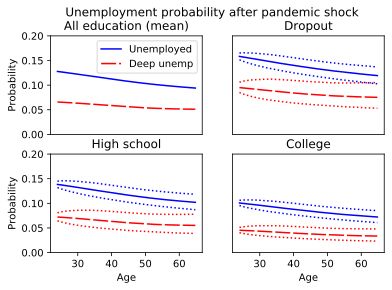
\includegraphics[width=\webWidth\textwidth]{./Figures/UnempProbByDemogBasic}
  } %\end{Web}
  { 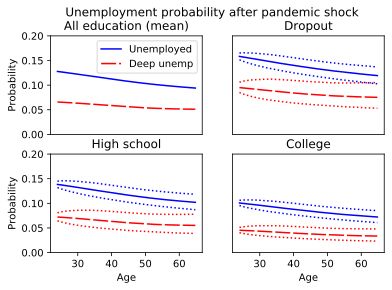
\includegraphics[width=0.8\textwidth]{./Figures/UnempProbByDemogBasic}}
\end{figure}


\subsubsection{The CARES Act}

We model the two elements of the CARES Act that directly affect the income of households:
\begin{itemize}
\item The stimulus check of \$1,200 for every adult taxpayer, means tested for previous years' income.\footnote{The act also includes \$500 for every child. In the model, an agent is somewhere between a household and an individual. While we do not model the \$500 payments to children, we also do not account for the fact that some adults will not receive a check. In aggregate we are close to the Joint Committee on Taxation's estimate of the total cost of the stimulus checks.}
\item The extra unemployment benefits of \$600 for up to 13 weeks, a total of \$7,800.
  For normal unemployed, we assume they receive only \$5,200 to reflect the idea that they may not be unemployed the entire 13 weeks.
\end{itemize}

We model the stimulus checks as being announced at the same time as the crisis hits.
However, only a quarter of households change their behavior immediately at the time of announcement, as calibrated to past experience.
The remainder do not respond until their stimulus check arrives, which we assume happens in the following quarter.
The households that pay close attention to the announcement of the policy are assumed to be so forward looking that they act as though the payment will arrive with certainty next period; the model even allows them to borrow against it if desired.\footnote{See \cite{carroll_sticky_2020} for a detailed discussion of the motivations behind this way of modeling stimulus payments, and a demonstration that this model matches the empirical evidence of how and when households have responded to stimulus checks in the past --- see \cite{psjmMPC2008}, \cite{brodaParker} and \cite{parker25million}, among others.  See also \cite{fhnMPC} for a natural experiment measured using national registry data.}

The extra unemployment benefits are assumed to both be announced and arrive at the beginning of the second quarter of 2020, and we assume that there is no delay in the response of unemployed households' consumption to these benefits.

\hypertarget{labor-income}{}
Figure~\ref{labor_income} shows the path of labor income --- exogenous in our model --- in the baseline and in the pandemic, both with and without the CARES Act.
Income in quarters Q2 and Q3 2020 is substantially boosted (by around 10 percent) by the extra unemployment benefits and the stimulus checks.
After two years, aggregate labor income is almost fully recovered.  See below for a brief discussion of analyses that attempt to endogenize labor supply and other equilibrium variables.

\begin{figure}
  \centering
  \caption{Labor and Transfer Income}
  \label{labor_income}
  % \begin{Web}
  \ifthenelse{\boolean{ifWeb}}{
    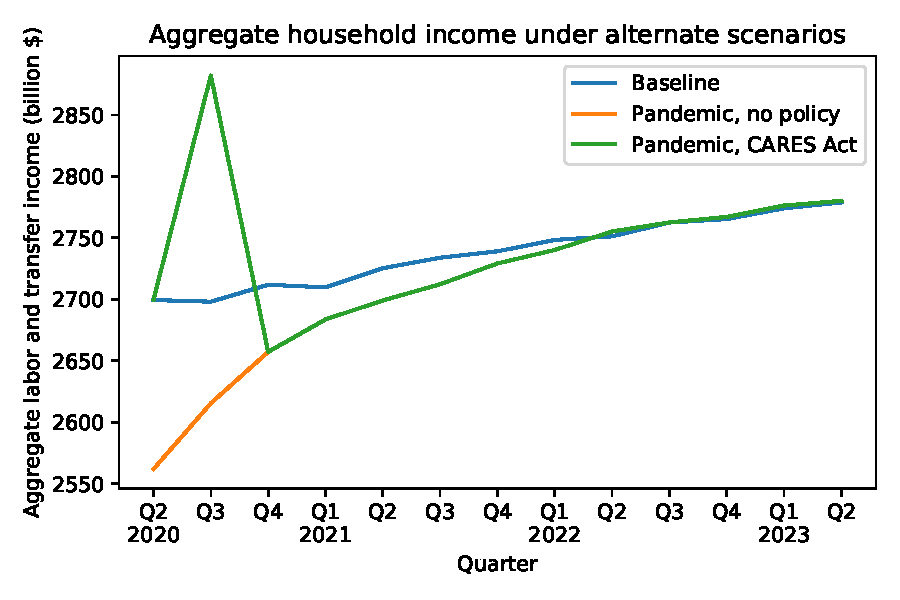
\includegraphics[width=\webWidth\textwidth]{./Figures/AggLT}
  } %\end{Web}
  { 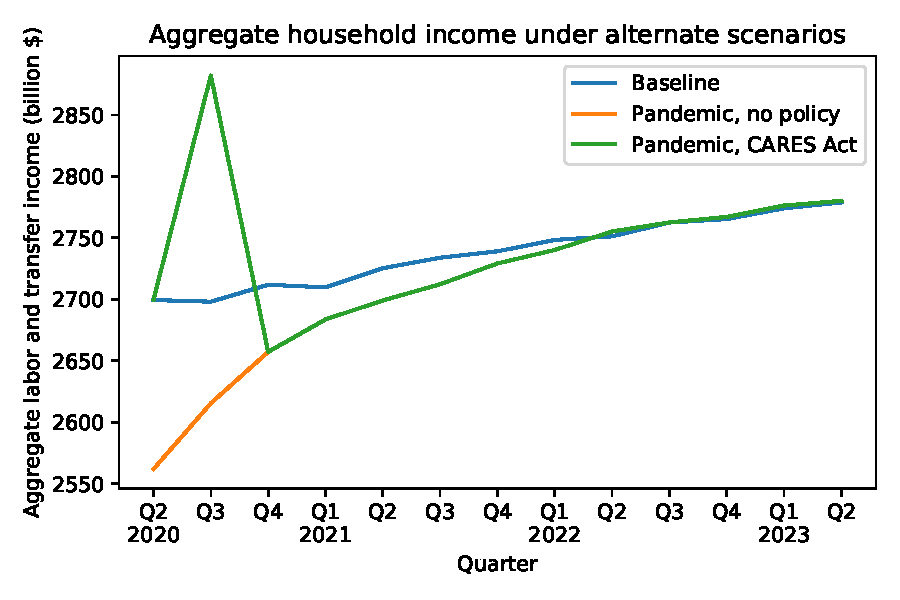
\includegraphics[width=0.8\textwidth]{./Figures/AggLT}}
\end{figure}


\hypertarget{Results}{}
\section{Results}

This section presents our simulation results for the scenario described above. In addition, we then model a more pessimistic scenario with a longer lockdown and higher initial unemployment rate.
\hypertarget{cons-response}{}

\begin{figure}
  \centering
  \caption{Consumption Response to the Pandemic and the Fiscal Stimulus}
  \label{cons_response}
  % \begin{Web}
  \ifthenelse{\boolean{ifWeb}}{
    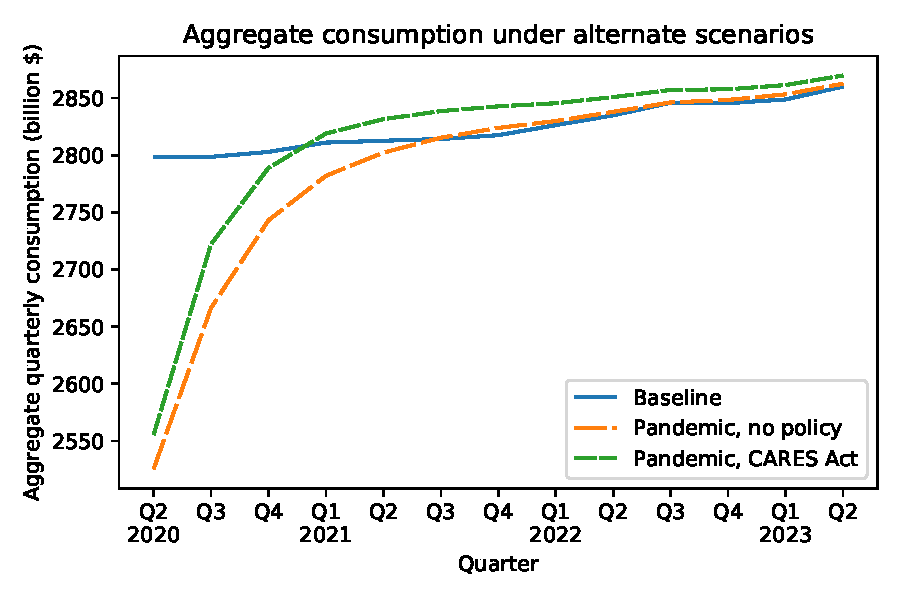
\includegraphics[width=\webWidth\textwidth]{./Figures/AggConResp_examples}
  } %\end{Web}
  { 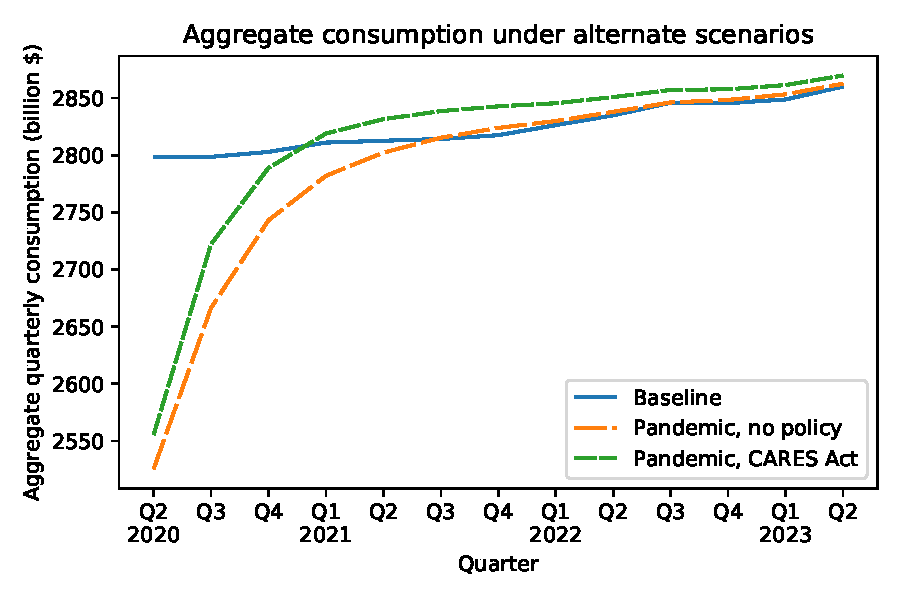
\includegraphics[width=0.8\textwidth]{./Figures/AggConResp_examples}}
\end{figure}

\subsection{Short-lived Pandemic}

Figure \ref{cons_response} shows three scenarios for quarterly aggregate consumption: (i) the baseline with no pandemic; (ii) the pandemic with no fiscal response; (iii) the pandemic with both the stimulus checks and extended unemployment benefits in the CARES Act.
The pandemic reduces consumption by ten percentage points in Q2 2020 relative to the baseline.

Without the CARES Act, consumption remains depressed through to the second half of 2021, at which point spending returns to the baseline level as a result of the buildup of liquid assets during the pandemic by households that do not lose their income.
We capture the limited spending options during the lockdown period by a reduction in the utility of consumption, which makes households save more during the pandemic than they otherwise would have, with the result that they build up liquid assets.
When the lockdown ends, the pent up savings of the always-employed become available to finance a resurgence in their spending, but the depressed spending of the two groups of unemployed people keeps total spending below the baseline until most of them are reemployed, at which point their spending (mostly) recovers while the always-employed are still spending down their extra savings built up during the lockdown.

Figure \ref{cons_response2} decomposes the effect of the pandemic on aggregate consumption (with no fiscal policy response), separating the drop in marginal utility from the reduction in income due to mass layoffs.
The figure illustrates that the constrained consumption choices are quantitatively key in capturing the expected depth in the slump of spending, which is already under way; see \cite{baker_Cpandemic} and \cite{nyFedCoronaBlog} for early evidence.
The marginal utility shock hits all households, and directly affects their spending decisions in the early quarters after the pandemic; its effect cannot be mitigated by fiscal stimulus.
The loss of income from unemployment is large, but affects only a fraction of households, who are disproportionately low income and thus account for a smaller share of aggregate consumption.
Moreover, most households hold at least some liquid assets, allowing them to smooth their consumption drop --- the 5 percent  decrease in labor income in Figure~\ref{labor_income} induces only a 1.5 percent decrease in consumption in Figure~\ref{cons_response2}.

\begin{figure}
  \centering
  \caption{Decomposition of Effect of the Pandemic on Aggregate Consumption (No Policy Response)}
  \label{cons_response2}
  % \begin{Web}
  \ifthenelse{\boolean{ifWeb}}{
    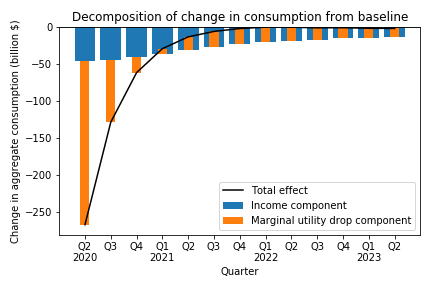
\includegraphics[width=\webWidth\textwidth]{./Figures/Decomposition}
  } %\end{Web}
  { 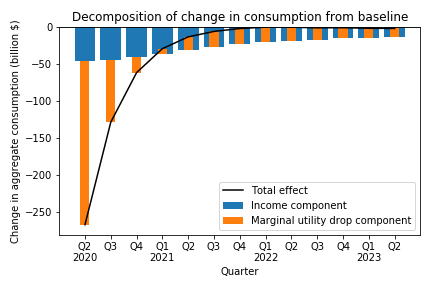
\includegraphics[width=0.8\textwidth]{./Figures/Decomposition}}
\end{figure}

Figure \ref{cons_response_emp} shows how the consumption response varies depending on the employment status of households in Q2 2020.
For each employment category (employed, unemployed, and deeply unemployed), the figure shows consumption relative to the same households' consumption in the baseline scenario with no pandemic (dotted lines).\footnote{Households that become unemployed during the pandemic might or might not have been unemployed otherwise. We assume that all households that would have been unemployed otherwise are either unemployed or deeply unemployed in the pandemic scenario. However, there are many more households that are unemployed in the pandemic scenario than in the baseline.}
The upper panel shows consumption without any policy response, while the lower panel includes the CARES Act.
The figure illustrates an important feature of the unemployment benefits that is lost at the aggregate level: the response provides the most relief to households whose consumption is most affected by the pandemic.
For the unemployed --- and especially for the deeply unemployed --- the consumption drop when the pandemic hits is much shallower and returns faster toward the baseline when the fiscal stimulus is in place.

\begin{figure}
  \centering
  \caption{Consumption Response by Employment Status}
  \label{cons_response_emp}
  % \begin{Web}
  \ifthenelse{\boolean{ifWeb}}{
    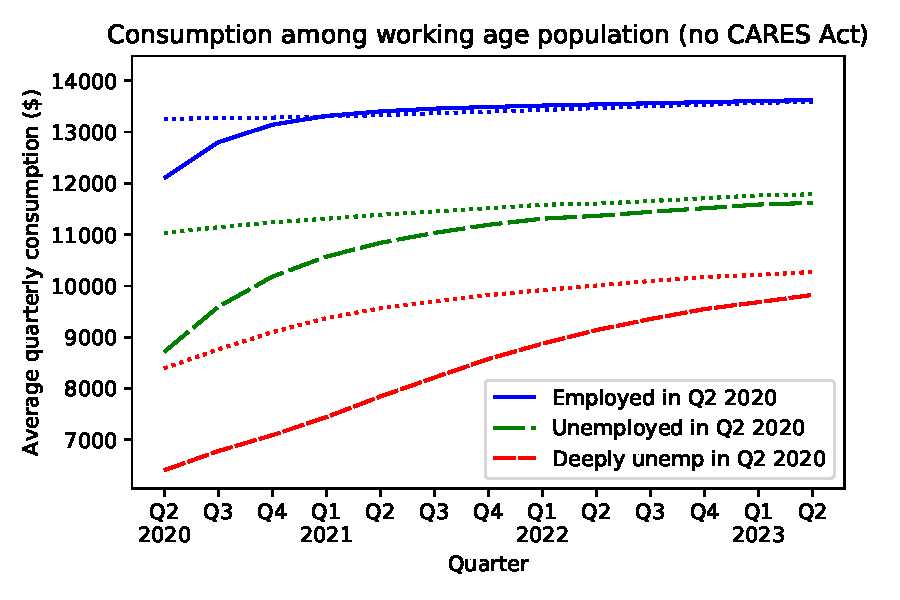
\includegraphics[width=0.8\webWidth\textwidth]{./Figures/ConRespByEmpStateNoStim}

    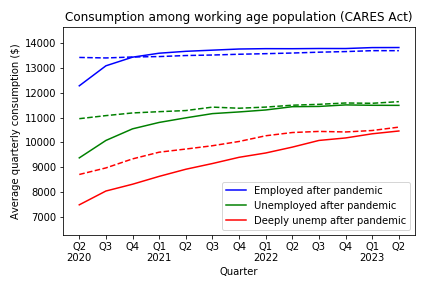
\includegraphics[width=0.8\webWidth\textwidth]{./Figures/ConRespByEmpStateWStim}
  } %\end{Web}
  { 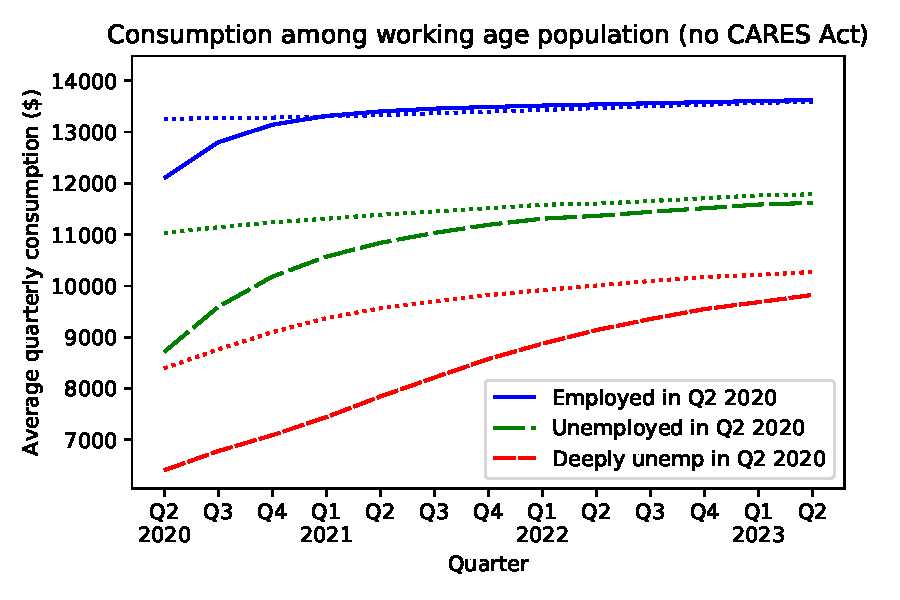
\includegraphics[width=0.8\textwidth]{./Figures/ConRespByEmpStateNoStim}
    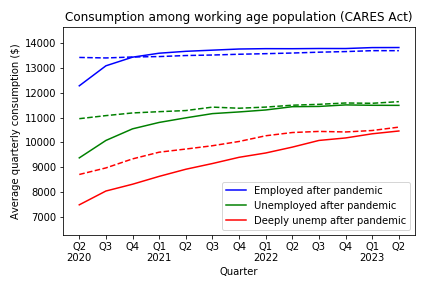
\includegraphics[width=0.8\textwidth]{./Figures/ConRespByEmpStateWStim}}
\end{figure}

Indeed, this targeted response is again seen in Figure~\ref{stim_by_emp},
showing the extra consumption relative to the pandemic scenario without the CARES Act.
The short-dashed and dotted lines show the effect of the stimulus check in isolation (for employed workers this is the same as the total fiscal response).
For unemployed households, this is dwarfed by the increased unemployment benefits.
These benefits both arrive earlier and are much larger.
Specifically, in Q3 2020, when households receive the stimulus checks, the effect of unemployment benefits on consumption makes up about 70 percent and 85 percent of the total effect for the normally and deeply unemployed, respectively.

\begin{figure}
  \centering
  \caption{Effect of CARES Act by Employment Status}
  \label{stim_by_emp}
  % \begin{Web}
  \ifthenelse{\boolean{ifWeb}}{
    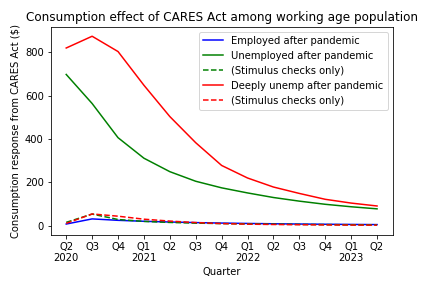
\includegraphics[width=\webWidth\textwidth]{./Figures/ConDeltaByEmpState}
  } %\end{Web}
  { 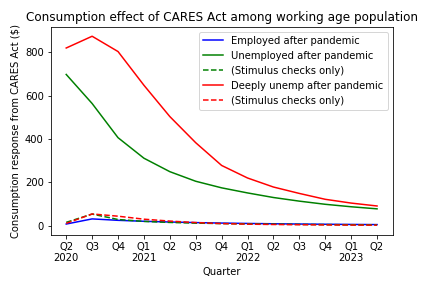
\includegraphics[width=0.8\textwidth]{./Figures/ConDeltaByEmpState}}
\end{figure}

Figure~\ref{checks_vs_unemp} aggregates the decomposition of the CARES Act in Figure~\ref{stim_by_emp} across all households.
In our model economy, the extra unemployment benefits amount to \$544 per household, while the stimulus checks amount to \$1,054 per household (as means testing reduces or eliminates the stimulus checks for high income households).
Aggregated, stimulus checks amount to \$267 billion, while the extended unemployment benefits amount to just over half that, \$137 billion.\footnote{See Appendix \ref{sec:aggregation} for details on how we aggregate households.}
The figure shows that during the peak consumption response in Q3 2020, the stimulus checks account for about 70~percent of the total effect on consumption for the average household and the unemployment benefits for about 30~percent.  Thus, although the unemployment benefits make a much larger difference to the spending of the individual recipients than the stimulus checks, a small enough proportion of households becomes unemployed that the total extra spending coming from these people is less than the total extra spending from the more widely distributed stimulus checks.

\begin{figure}
  \centering
  \caption{Aggregate Consumption Effect of Stimulus Checks vs Unemployment Benefits}
  \label{checks_vs_unemp}
  % \begin{Web}
  \ifthenelse{\boolean{ifWeb}}{
    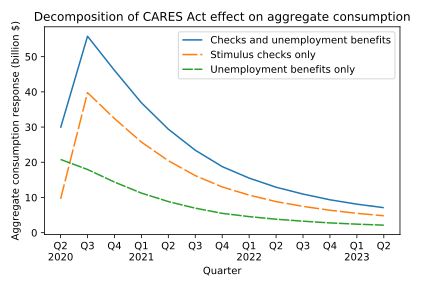
\includegraphics[width=\webWidth\textwidth]{./Figures/Checks_vs_Unemp}
  } %\end{Web}
  { 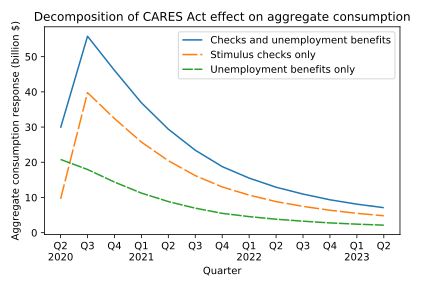
\includegraphics[width=0.8\textwidth]{./Figures/Checks_vs_Unemp}}
\end{figure}

The previous graphs show the importance of the targeted unemployment benefits at the individual level, but the aggregate effect is less striking.
Figure~\ref{EffectTargeting} compares the effect of the CARES Act (both unemployment insurance and stimulus checks) to a policy of the same absolute size that distributes checks to everybody.
While unemployment benefits arrive sooner, resulting in higher aggregate consumption in Q2 2020, the un-targeted policy leads to higher aggregate consumption in the following quarters.

The interesting conclusion is that, while the net spending response is similar for alternative ways of distributing the funds, the choice to extend unemployment benefits means that much more of the extra spending is coming from the people who will be worst hurt by the crisis.  This has obvious implications for the design of any further stimulus packages that might be necessary if the crisis lasts longer than our baseline scenario assumes.

\begin{figure}
  \centering
  \caption{Effect of Targeting the CARES Act Consumption Stimulus}
  \label{EffectTargeting}
  % \begin{Web}
  \ifthenelse{\boolean{ifWeb}}{
    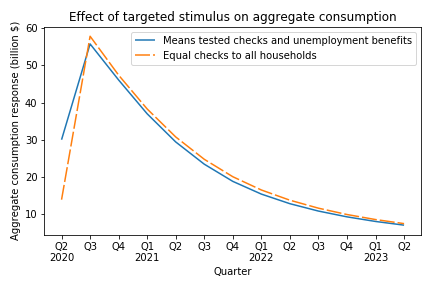
\includegraphics[width=\webWidth\textwidth]{./Figures/EffectTargeting}
  } %\end{Web}
  { 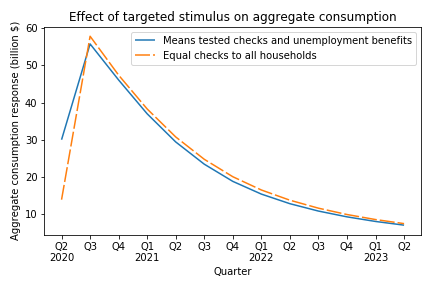
\includegraphics[width=0.8\textwidth]{./Figures/EffectTargeting}}
\end{figure}


\subsection{Alternative Scenario: Long, Deep Pandemic} \label{sec:longPandemic}

Given the uncertainty about how long and deep the current recession will be, we investigate a more pessimistic scenario in which the lockdown is expected to last for four quarters.
In addition, the unemployment rate increases to 20 percent in Q2 2020, consisting of 15 percent of deeply unemployed and 5 percent of normal unemployed.
In this scenario we compare how effectively the CARES package stimulates consumption, also considering a more generous plan in which the unemployment benefits continue until the lockdown is over.
We model the receipt of unemployment benefits each quarter as an unexpected shock, representing a series of policy renewals.

\begin{figure}
  \centering
  \caption{Labor and Transfer Income During the Long, Four-Quarter Pandemic}
  \label{inc_response_pandemic}
  % \begin{Web}
  \ifthenelse{\boolean{ifWeb}}{
    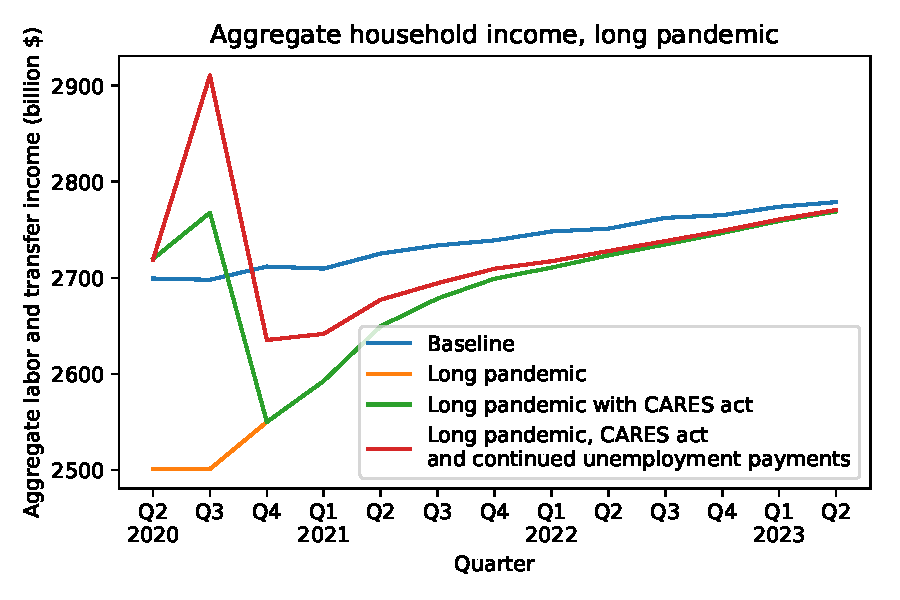
\includegraphics[width=\webWidth\textwidth]{./Figures/AggLT_long_pandemic}
  } %\end{Web}
  { 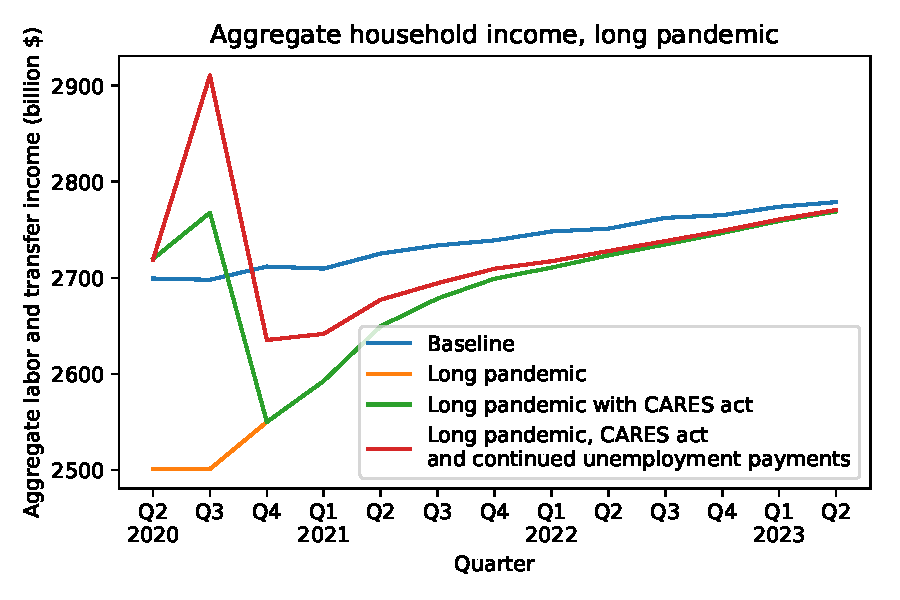
\includegraphics[width=0.8\textwidth]{./Figures/AggLT_long_pandemic}}
\end{figure}

Figure~\ref{inc_response_pandemic} compares the effects of the two fiscal stimulus policies on income.
The persistently high unemployment results in a substantial and long drop in aggregate income (long-dashed) as compared to the no pandemic scenario.
The CARES stimulus (medium-dashed) provides only a short term support to income for the first two quarters.
In contrast, the scenario with unemployment benefits extended as long as the lockdown lasts (dotted) keeps aggregate income elevated through the recession.

\begin{figure}
  \centering
  \caption{Consumption Response to the Long, Four-Quarter Pandemic}
  \label{cons_response_pandemic}
  % \begin{Web}
  \ifthenelse{\boolean{ifWeb}}{
    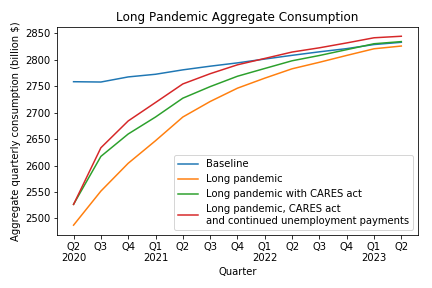
\includegraphics[width=\webWidth\textwidth]{./Figures/DeepPandemic}
  } %\end{Web}
  { 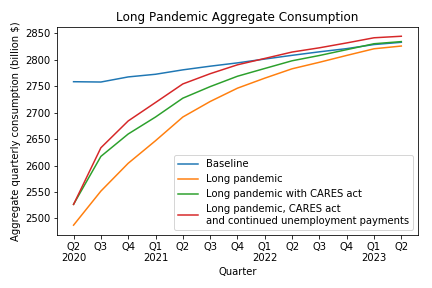
\includegraphics[width=0.8\textwidth]{./Figures/DeepPandemic}}
\end{figure}

Figure~\ref{cons_response_pandemic} shows the implications of the two stimulus packages for aggregate consumption.
The long lockdown causes a much longer decline in spending than the shorter lockdown in our primary scenario. In the shorter pandemic scenario (Figure~\ref{cons_response}) consumption returns to the baseline path after roughly one year, while in the long lockdown shown here the recovery takes around three years;
the CARES stimulus shortens the consumption drop to about two years.
The scenario with extended unemployment benefits ensures that aggregate spending returns to near the baseline path after just over one year, and does so by targeting the funds to the people who are worst hurt by the crisis and to whom the cash will make the most difference.

\section{Conclusions}

Our model suggests that there may be a strong consumption recovery when the social-distancing requirements of the pandemic begin to subside.
We invite readers to test the robustness of this conclusion by using the associated software toolkit to choose their own preferred assumptions on the path of the pandemic, and of unemployment, to understand better how consumption will respond.

One important limitation of our analysis is that it does not incorporate Keynesian demand effects or other general equilibrium responses to the consumption fluctuations we predict.
In practice, Keynesian effects are likely to cause movements in aggregate income in the same direction as consumption; in that sense, our estimates can be thought of as a ``first round'' analysis of the dynamics of the crisis, which will be amplified by any Keynesian response.  (See \cite{bayer_corona} for estimates of the multiplier for transfer payments).
These considerations further strengthen the case that the CARES Act will make a substantial difference to the economic outcome.
A particularly important consideration is that forward-looking firms that expect consumer demand to return forcefully in the third and fourth quarters of 2020 are more likely to maintain relations with their employees so that they can restart production quickly.

The ability to incorporate Keynesian demand effects is one of the most impressive achievements of the generation of heterogeneous agent macroeconomic models that have been constructed in the last few years.
But the technical challenges of constructing those models are such that they cannot yet incorporate realistic treatments of features that our model says are quantitatively important, particularly differing risks of (and types of) unemployment, for different kinds of people (young, old; rich, poor; high- and low-education).
This rich heterogeneity is important both to the overall response to the CARES Act, and to making judgments about the extent to which it has been successfully targeted to provide benefits to those who need them most.
A fuller analysis that incorporates such heterogeneity, which is of intrinsic interest to policymakers, as well as a satisfying treatment of general equilibrium will have to wait for another day, but that day is likely not far off.


\pagebreak

\small
\bibliography{LaTeX/\texname,LaTeX/\texname-Add,\economics}
\normalsize

\ifthenelse{\boolean{ifIJCB}}{\processdelayedfloats}{} 

\pagebreak
\appendix
\setcounter{table}{0}
\renewcommand{\thetable}{A\arabic{table}}

% Redefine so that things that should be done only in the subfile are not done
% when reading it as part of the main file
\renewcommand{\onlyinsubfile}[1]{}
\renewcommand{\notinsubfile}[1]{#1}

\subfile{ModelAppendix}

% \begin{Web}
\ifthenelse{\boolean{ifWeb}}{
  \newpage
  \printendnotes[superscriptednotes]
}{}
% \end{Web}


\end{document}
% Config for AucTeX on MacOS using Skim as previewer 
% Local Variables:
% TeX-PDF-mode: t
% TeX-file-line-error: t
% TeX-command-extra-options: "-output-directory=LaTeX -shell-escape -interaction=nonstopmode -synctex=1"
% eval: (setq TeX-command-list  (remove '("BibTeX" "%(bibtex) %s" TeX-run-BibTeX nil t :help "Run BibTeX") TeX-command-list))
% eval: (add-to-list 'TeX-command-list	'("BibTeX" "bibtex LaTeX/%s" TeX-run-BibTeX nil t :help "Run BibTeX") t)
% eval: (setq TeX-view-program-selection '((output-pdf "Skim")))
% eval: (setq TeX-view-program-list '(("Skim" "/Applications/Skim.app/Contents/SharedSupport/displayline -b -g %n LaTeX/%o %b")))
% LaTeX-command-style: (("" "%(PDF)%(latex) %(file-line-error) %(extraopts) %S%(PDFout)"))
% TeX-source-correlate-mode: t
% TeX-source-correlate-start-server: 0
% End:
